In accordance with our goal of language agnosticism, \textit{libinger} exposes both C
and Rust~\cite{www-rustlang} APIs.  To demonstrate the flexibility and composability
of the preemptible function abstraction, we have also created \textit{libturquoise},
a preemptive userland thread library for Rust, by porting an existing futures-based
thread
pool to \textit{libinger}.  We discuss this system in \Chap~\ref{sec:libturquoise}.

Figure~\ref{fig:architecture} shows a dependency graph of the software components
comprising the preemptible functions stack.  The \textit{libinger} library itself is
implemented in approximately 2,500 lines of Rust.  To support calls to nonreentrant
functions, it depends on another library, \textit{libgotcha}, which consists of
another 3,000 lines of C, Rust, and x86-64 assembly.  We cover the details in
\Chap~\ref{sec:libgotcha}.

\begin{figure}
\begin{center}
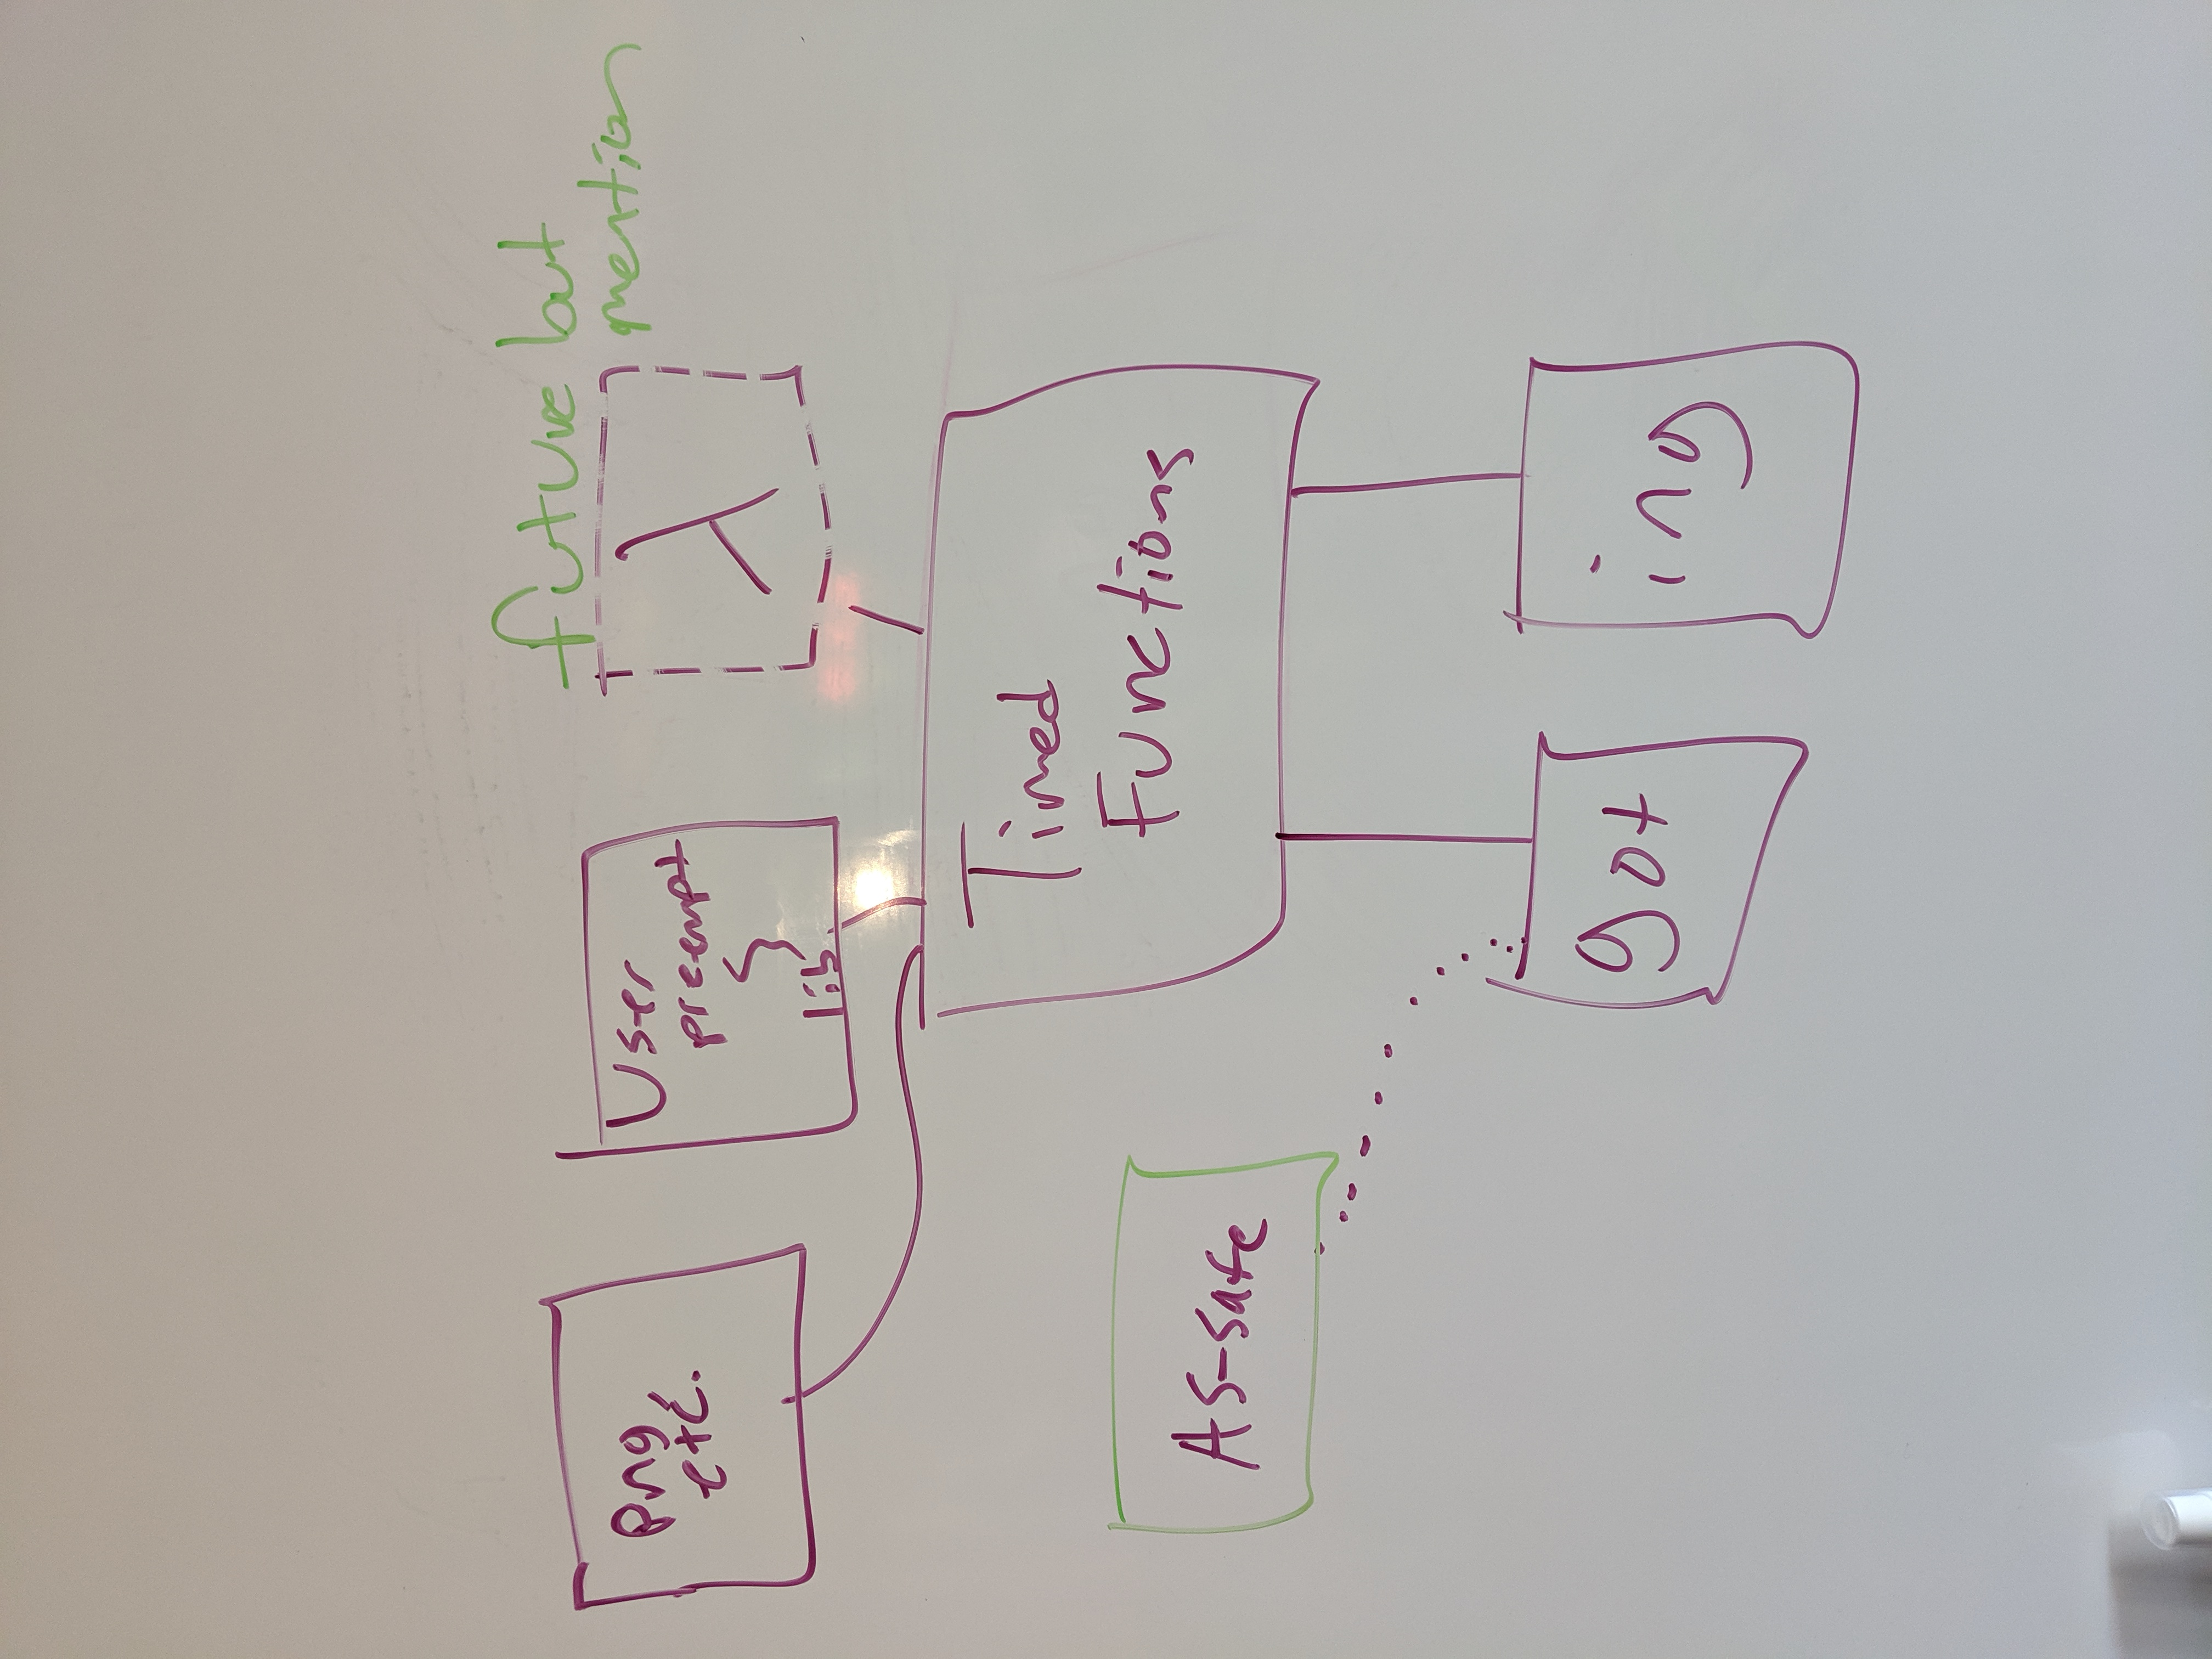
\includegraphics[width=\columnwidth]{figs/architecture}
\end{center}
\caption{Preemptible functions software stack.  \textnormal{Hexagonal boxes show
the required runtime environment.  Rectangular boxes represent components
implementing the preemptible functions abstraction.  Ovals represent components built
on top of these.  A preemptible function's body (i.e., \texttt{func}) may be defined
directly in
your program, or in some other loaded library.}}
\label{fig:architecture}
\end{figure}
